\section{Results and Analysis}
\label{sec:experiment}
\subsection{Effect of Demonstrations on Fine-tuned GPT-2}

We manually design two templates to form the addition problems, where [x1], [x2] and [y] in the templates will be filled in with numbers.

\begin{itemize}
\item Template 1: " [x1] + [x2] = [y]"
\item Template 2: "[x1]+[x2]=[y]".
\end{itemize}

Template 1 differs from template 2 in that the former puts an additional space before each number. The intuition of adding a space is that GPT-2 uses BPE tokenization which will consider the word begins with a space and the same word without a space as two different tokens. For instance, "1" and " 1" are two different tokens.

We list the experiment results on addition in \tabref{tbl:overall_res}. For a given number of demonstrations, we repeat the experiments for 25 times and report the mean and standard deviation of models' accuracy. From these results, we can see that for both fine-tuning methods, using template 1 (adding a space before each number) is helpful for both models. We assume that this difference may be caused by tokenization. As in our dataset, there exist up to 6-digit addition questions and the model will tokenize a 6-digit number into several tokens. In this case, when faced with a number of "123456",  the model trained with template 1 will regard it as " 123" and "456". While the second model will treat it as "123", "456". This is more difficult for the model to realize what is the beginning of the number and thus is more difficult to align the different number is the question, which will result in a worse performance in long digit additions consists of more than 2 tokens. A careful analysis of the result confirms our hypothesis, since for models trained via causal language modeling, the model achieves 16\% on 6-digit plus 6-digit problems if it uses the template 1, whereas this accuracy is 0\% if it uses the template 2.

% Another possible reason is that the numbers that begin with a space are abundant in the pretraining data of GPT2

We observe that in each of these two templates, adding demonstrations brings further improvements for model finetuned via causal language modeling, while for vanilla finetuned models this technique is detrimental. We attribute the cause of this phenomenon to the gap between training and testing. For vanilla finetuned model, there isn't any demonstrations in the context of its training instances, which may hinder the model from making better use of the demonstrations at inference time. On the other hand, the model finetuned via causal language modeling will try to predict every token in each of the 512-token long training instances. Since each of these training instances consists of multiple questions, thus the model is familiar with the task of predicting the answer given certain number of demonstrations, resulting in the improvements in the accuracy. We also notice that the accuracies between different numbers of demonstrations are stable for the model finetuned via causal language modeling, suggesting the improvements elicited by the demonstrations have an upper limit.

\begin{table}[h]
\begin{center}
\begin{small}
\begin{tabular}{ccc}
Types              & Template 1 & Template 2 \\
\toprule
Vanilla + 0 demo   & 25.8       & 1.4        \\
Vanilla + 1 demo   & 0.2 ± 0.2  & 0.0 ± 0.0  \\
Vanilla + 2 demo   & 0.0 ± 0.0  & 0.0 ± 0.0  \\
Vanilla + 3 demo   & 0.0 ± 0.0  & 0.0 ± 0.0  \\
\midrule
Causal LM + 0 demo & 18.4       & 1.8        \\
Causal LM + 1 demo & 47.5 ± 0.4 & 25.4 ± 0.4 \\
Causal LM + 2 demo & 47.3 ± 0.9 & 25.4 ± 0.8 \\
Causal LM + 3 demo & 47.3 ± 0.4 & 25.8 ± 0.6
\end{tabular}
\caption{\label{tbl:overall_res} Accuracy (in percentage) for models with different finetune method on addition. We also show models' accuracy given different number of demonstrations. Each setting is repeated 25 times to get the mean and standard deviation.}
\end{small}
\end{center}
\end{table}


%Moreover, in the non-ensemble scenario, we can see that the number of demonstrations has little impact on the overall accuracy, as the mean accuracy for different number of demonstrations are quite close. Meanwhile, although the standard deviation is relatively high among all the results with the same number of demonstrations, it’s stable within the same type of demonstrations as shown in \tabref{tbl:detailed_arith} and table \tabref{tbl:detailed_asdiv}. \textbf{This suggests that given a prompt consisting of some specific types of demonstrations, the model will give rather stable predictions. However, when the composition of the given prompt is different, the model will tend to make different predictions.}


\subsection{Effect of the Types of Demonstrations}

In this setting, we test the models on 500 questions of 3 digit plus 3 digit. We enumerate all 36 possible scenarios for 6-digit addition, i.e. the two numbers are chosen from 1 digit to 6 digit. For each of this scenario, we randomly choose 5 demonstrations and prompt the model with 1 demonstration at a time. We report the mean accuracy of each scenario in \figref{fig:diff-digits}.

The results show that the model will produce rather robust predictions regardless of the type of questions, as the difference between the max accuracy and the min accuracy is 1.6\% for template 1 and 3.9\%. We also notice that if the demonstration contains a small digit addition problem, like 1 digit plus 1 digit, the results are generally worse than the results given by a demonstration which contain large digit addition. We think this may due to the fact that small digits addition problem are relatively scarce in the training dataset, making them appear less frequently in the context during training. 

\begin{figure}[!htb]
   \begin{minipage}{0.49\textwidth}
     \centering
     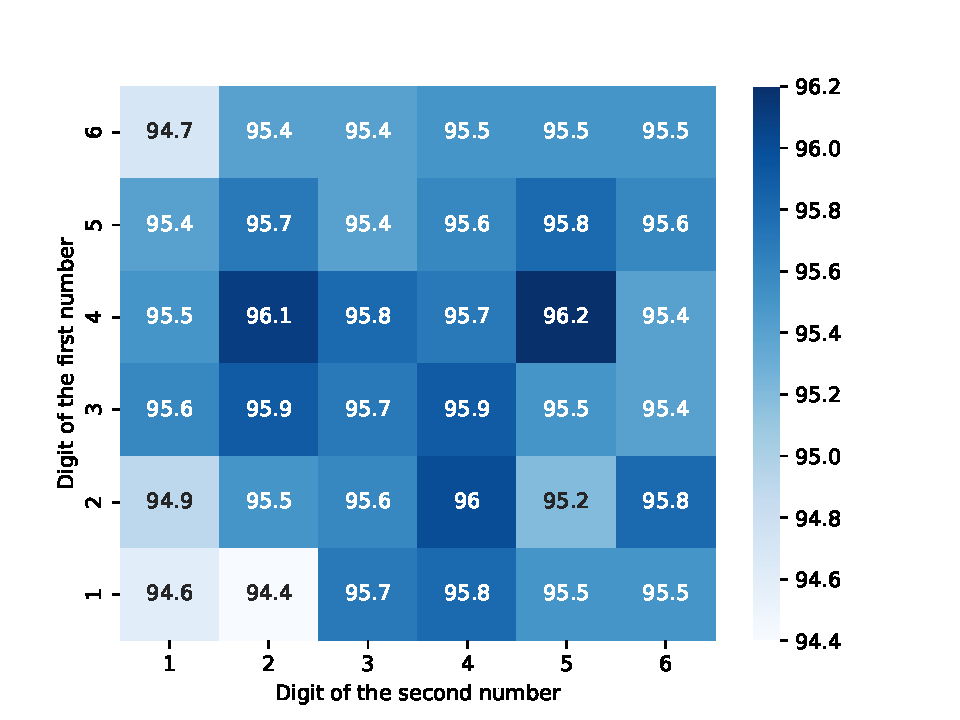
\includegraphics[width=.8\linewidth]{figs/gpt2-CLM-with-spaces-4e-DIFF-DIGITS.pdf}
%     \caption{Interpolation for Data 1}\label{Fig:Data1}
   \end{minipage}\hfill
   \begin{minipage}{0.49\textwidth}
     \centering
     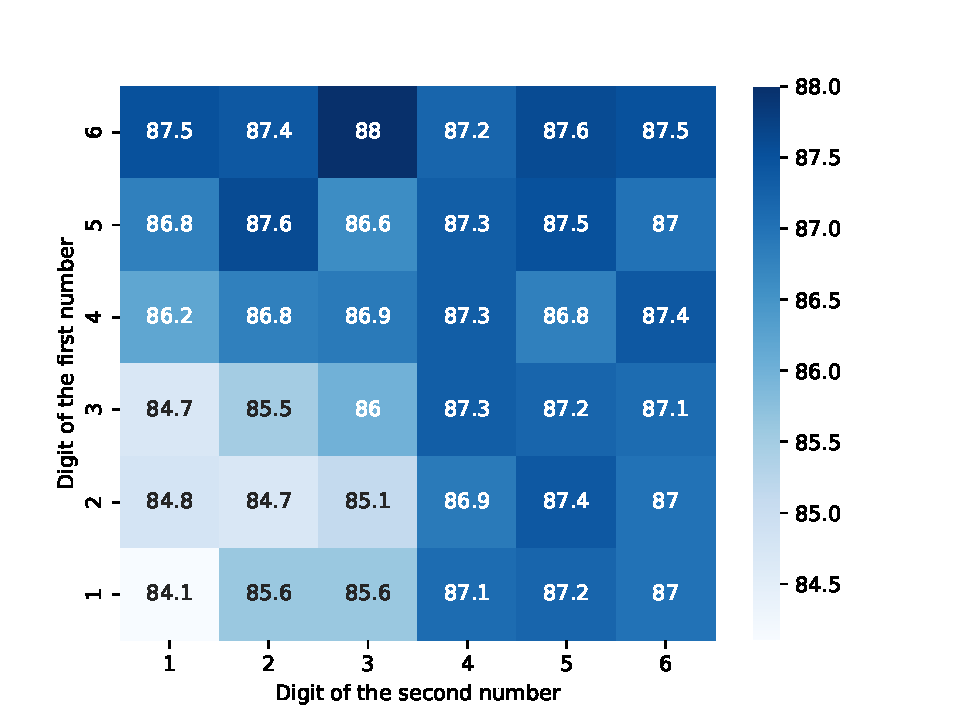
\includegraphics[width=.8\linewidth]{figs/gpt2-CLM-without-spaces-4e-DIFF-DIGITS.pdf}
%     \caption{Interpolation for Data 2}\label{Fig:Data2}
   \end{minipage}
       \caption{Effect of different types of demonstrations on the accuracy of 3-digit addition. Above: result for the model trained with template 1. Below: result for the model trained with template 2.}\label{fig:diff-digits}
\end{figure}

% \KZ{Put the two matrices horizontally side by side to save space. May need to enlarge the font in the matrices a bit.}

%\begin{figure}[th]
%\begin{center}
%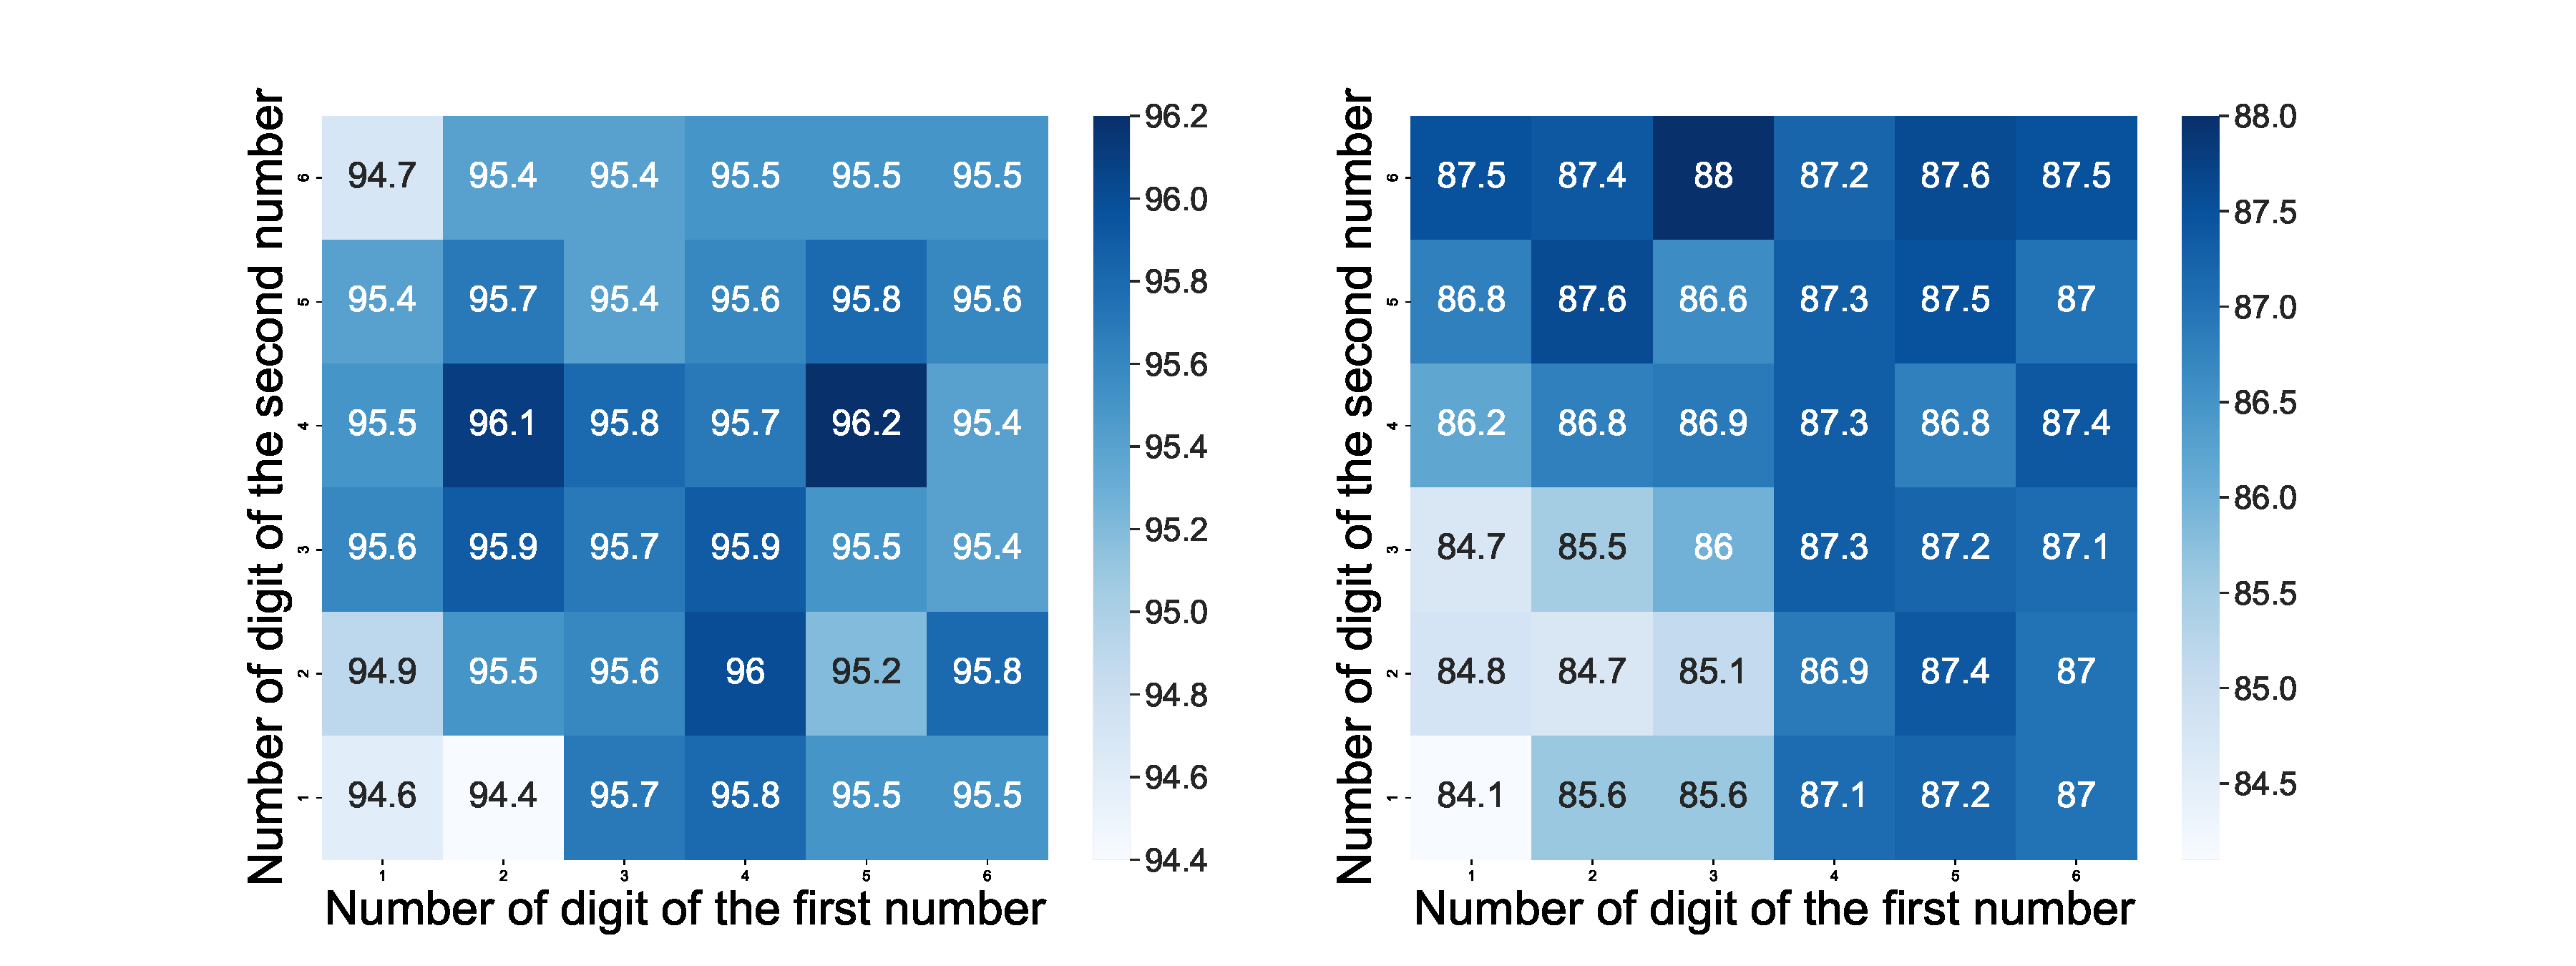
\includegraphics[width = \columnwidth]{figs/cmp-DIFF-DIGITS.pdf}
%\caption{Effect of different types of demonstrations on the accuracy of 3-digit addition. Left: result for the model trained with template 1. Right: result for the model trained with template 2.}
% \label{fig:diff-digits}
%\end{center}
%\end{figure}


\subsection{Effect of the Order of Demonstrations}
Prior work~\cite{order} has shown that LLMs are highly sensitive to the order of demonstrations. 
In this subsection, we study the sensitivity of fine-tuned GPT-2 on the order of in-context demonstrations.

For each trial, we randomly sample 4 demonstrations of 3 digit plus 3 digit questions. Then we test all of their permutations on the language model and calculate the difference between the max accuracy and the min accuracy among the 24 results. The accuracy difference is shown in \figref{fig:perm}. The results show that in both cases the difference is around 1.5\% for template 1 and 2.5\% for template 2, which suggest that models' predictions are relatively stable regardless of the order of demonstrations.


%\begin{figure}[!htb]
%   \begin{minipage}{0.49\textwidth}
%     \centering
%     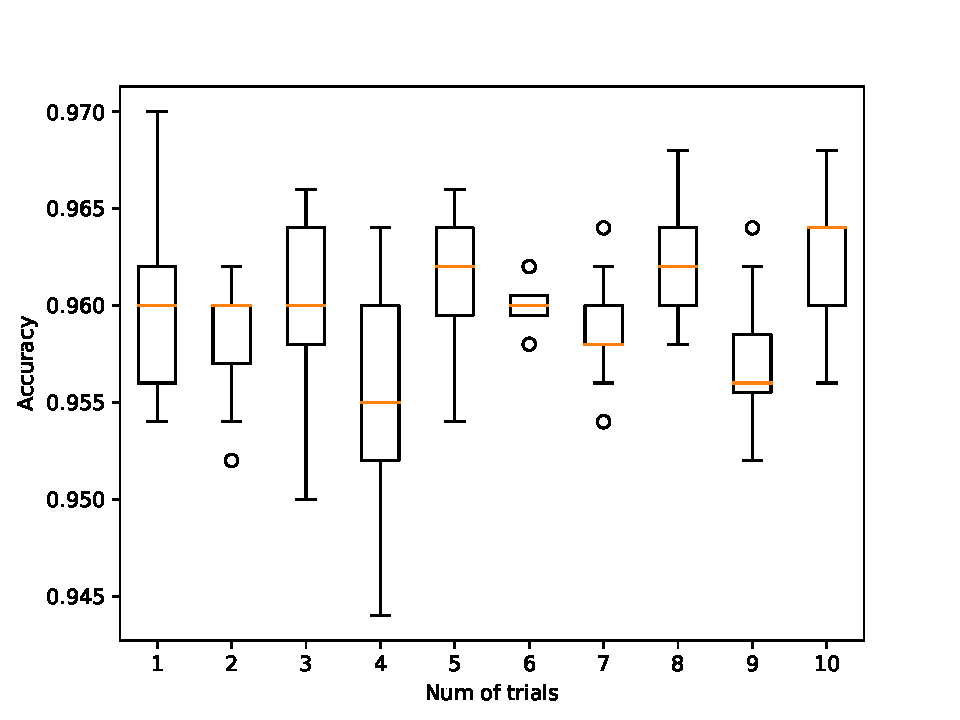
\includegraphics[width=.8\linewidth]{figs/gpt2-CLM-with-spaces-4e-PERM-4.pdf}
%%     \caption{Interpolation for Data 1}\label{Fig:Data1}
%   \end{minipage}\hfill
%   \begin{minipage}{0.49\textwidth}
%     \centering
%     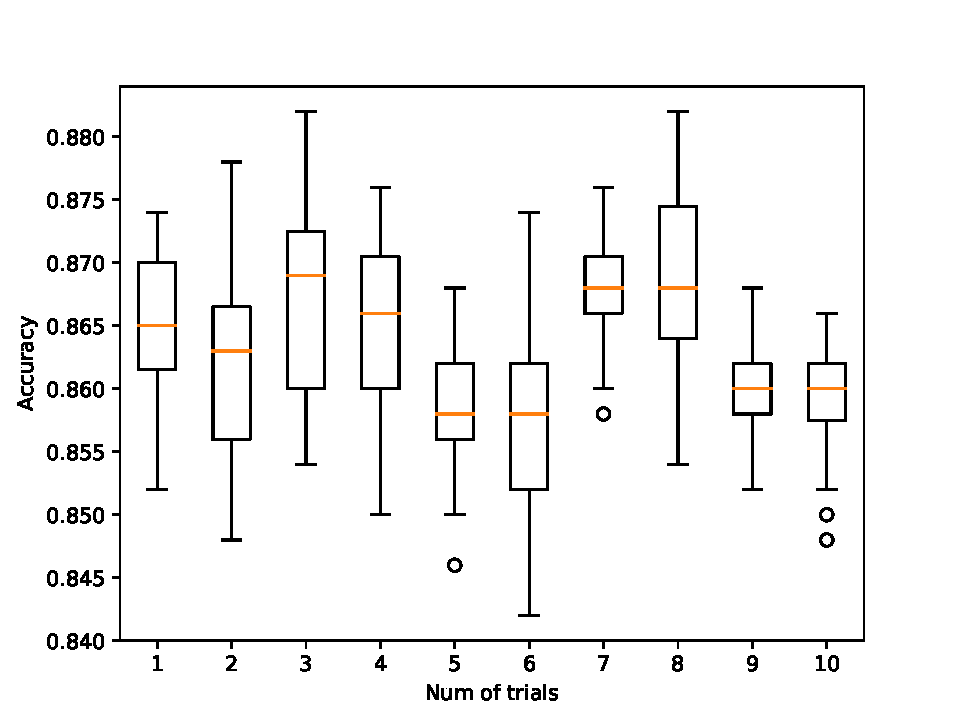
\includegraphics[width=.8\linewidth]{figs/gpt2-CLM-without-spaces-4e-PERM-4.pdf}
%%     \caption{Interpolation for Data 2}\label{Fig:Data2}
%   \end{minipage}
%       \caption{Effect of the order of demonstrations on the accuracy of 3-digit addition. Above: result for the model trained with template 1. Below: result for the model trained with template 2. \KZ{The x-axis should be called
%``trials'' rather than number of trials.}}\label{fig:perm}
%\end{figure}

\begin{figure}[th]
\begin{center}
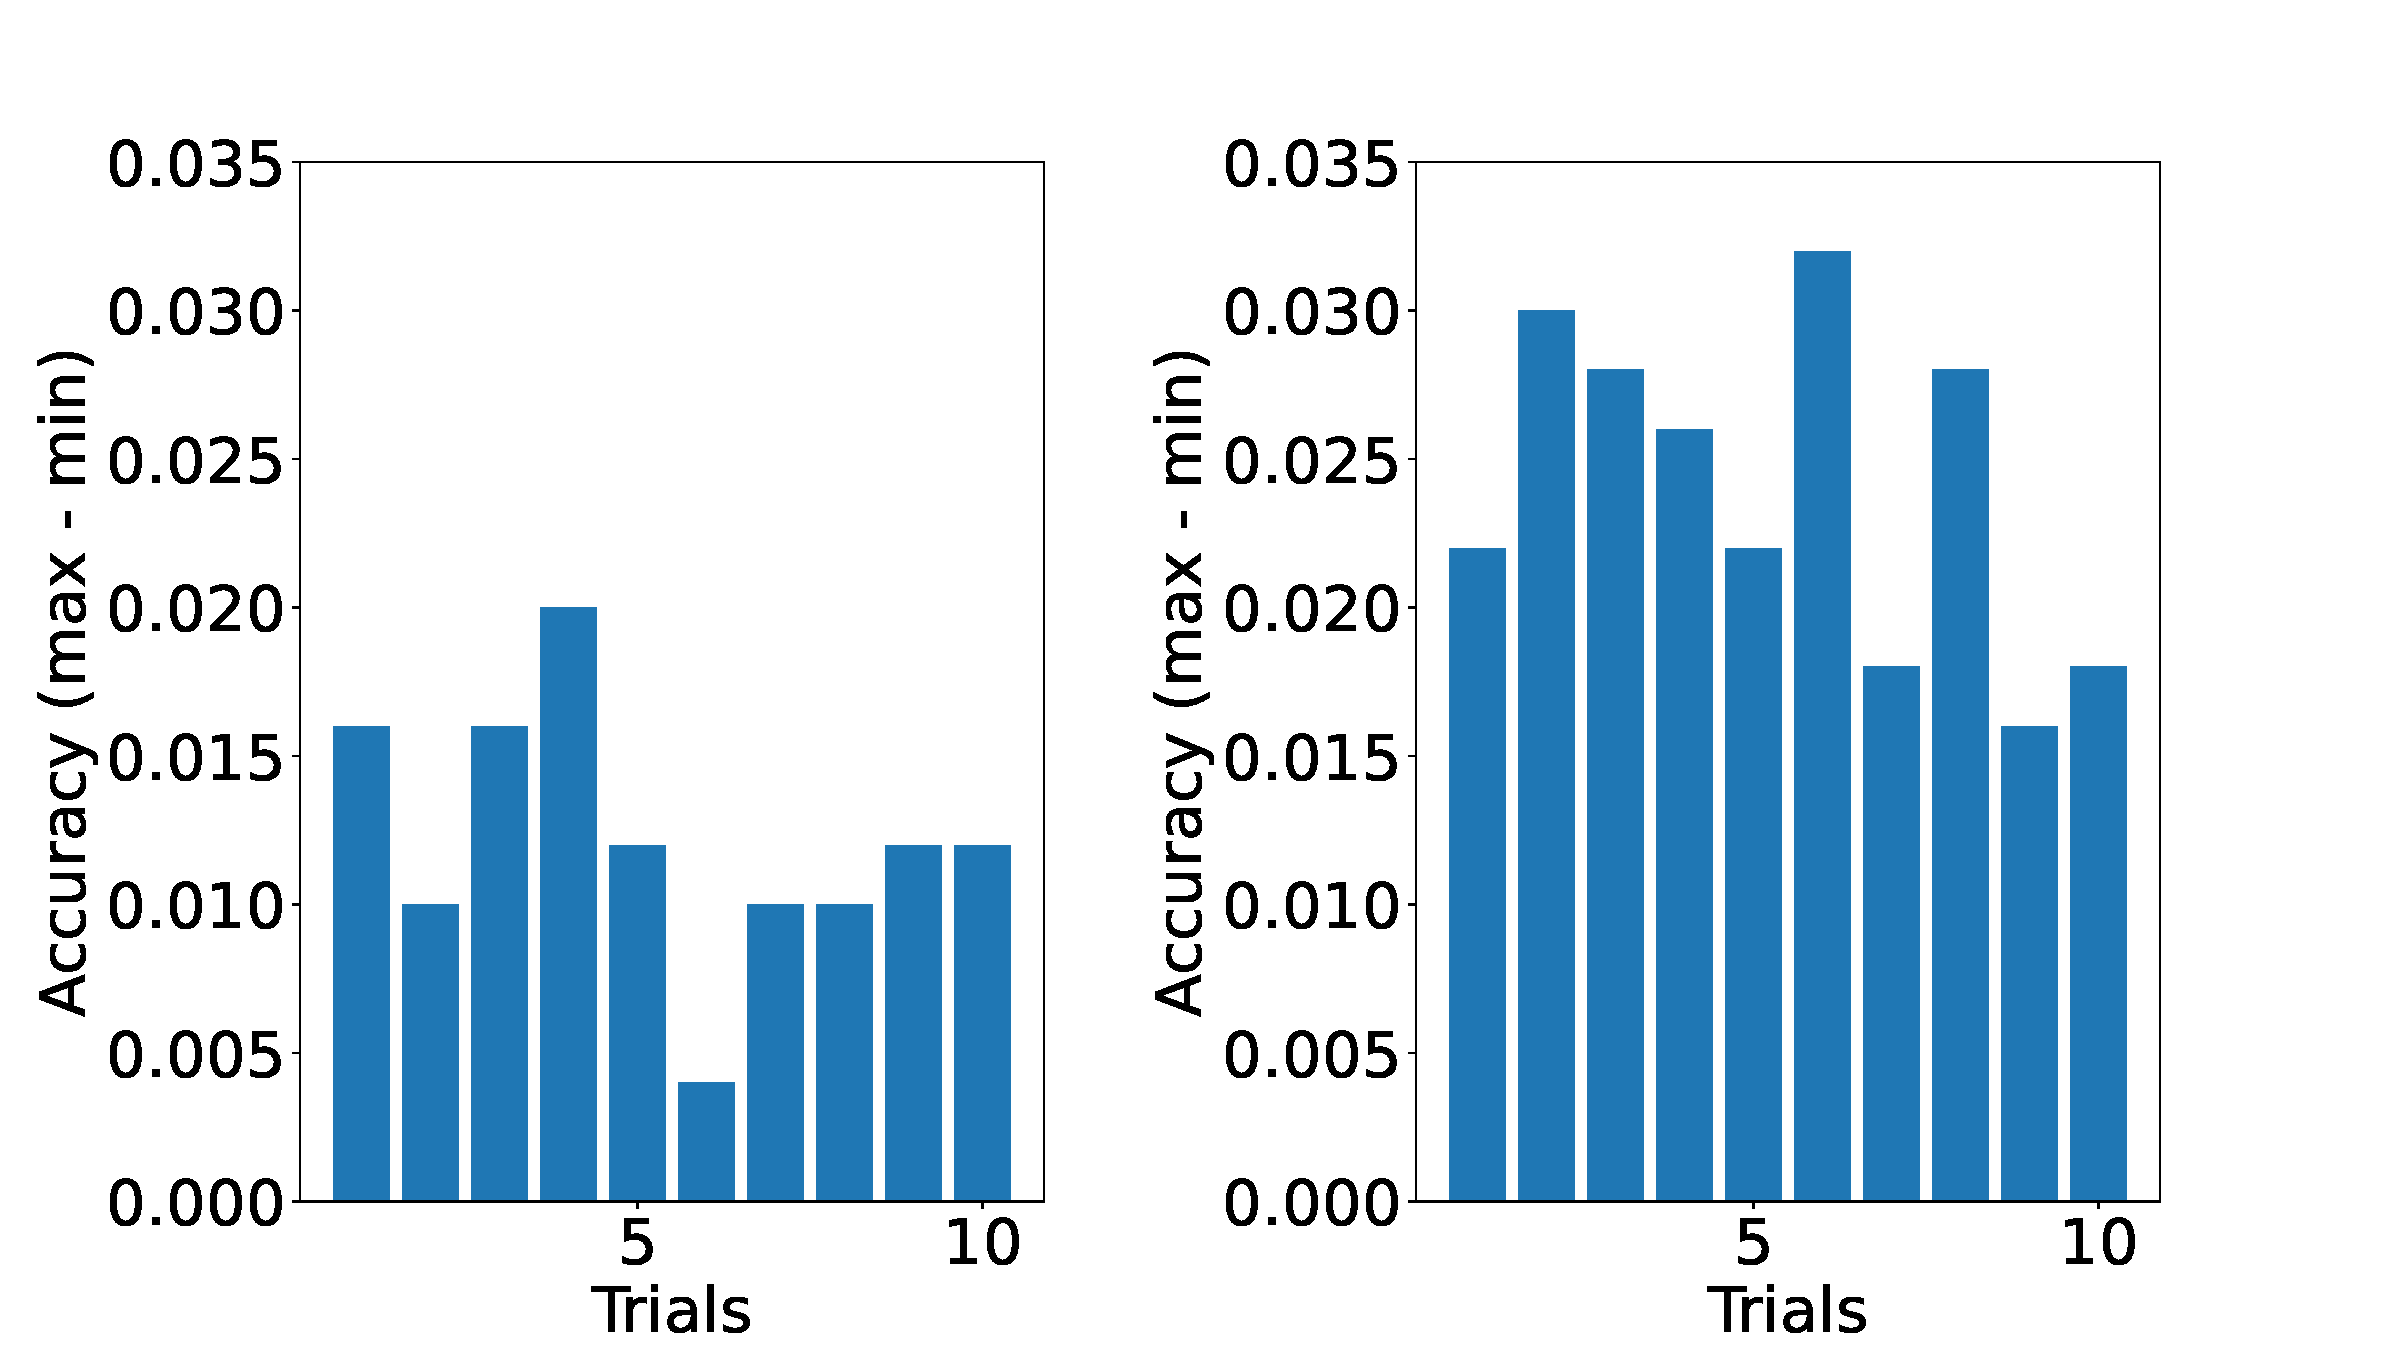
\includegraphics[width = \columnwidth]{figs/cmp-PERM.pdf}
\caption{Effect of the order of demonstrations on the accuracy of 3-digit addition, here we show the difference between the max accuracy and the min accuracy. Left: result for the model trained with template 1. Right: result for the model trained with template 2.}
 \label{fig:perm}
\end{center}
\end{figure}

